\documentclass[11pt]{article}

% ---------------------------------------------------------------------
% Packages
% ---------------------------------------------------------------------
\usepackage[a4paper,margin=2.4cm,headheight=14pt]{geometry}
\usepackage{textcomp}
\usepackage{amsmath,amssymb}
\usepackage{booktabs}
\usepackage{array}
\usepackage{longtable}
\usepackage{tabularx}
\usepackage{enumitem}
\usepackage{xcolor}
\usepackage{tikz}
\usetikzlibrary{arrows.meta,positioning}
\usepackage{fancyhdr}
\usepackage{titlesec}
\usepackage{parskip}
\usepackage{caption}
\usepackage{etoolbox}
\usepackage[colorlinks=true,linkcolor=armblue,urlcolor=armblue,citecolor=armblue,linktoc=all]{hyperref}

% ---------------------------------------------------------------------
% Palette + type
% ---------------------------------------------------------------------
\definecolor{armblue}{HTML}{1B44C4}
\definecolor{armgrey}{HTML}{565E70}
\definecolor{armrule}{HTML}{D6DAE3}
\definecolor{armok}{HTML}{166B45}
\definecolor{armwarn}{HTML}{95620A}
\definecolor{armbad}{HTML}{A8332A}

\newcommand{\code}[1]{\texttt{\detokenize{#1}}}
\newcommand{\degsym}{\ifmmode{}^{\circ}\else°\fi}
\newcommand{\micro}{\ifmmode\text{µ}\else µ\fi}
\newcolumntype{L}[1]{>{\raggedright\arraybackslash}p{#1}}
\newcommand{\okmark}{\textcolor{armok}{\textbf{OK}}}
\newcommand{\warnmark}{\textcolor{armwarn}{\textbf{watch}}}
\newcommand{\badmark}{\textcolor{armbad}{\textbf{fails}}}

\titleformat{\section}{\normalfont\Large\bfseries\color{armblue}}{\thesection}{0.6em}{}[{\color{armrule}\titlerule}]
\titleformat{\subsection}{\normalfont\large\bfseries}{\thesubsection}{0.6em}{}
\titlespacing*{\section}{0pt}{1.6em}{0.8em}
\titlespacing*{\subsection}{0pt}{1.2em}{0.5em}

\pagestyle{fancy}
\fancyhf{}
\renewcommand{\headrulewidth}{0.4pt}
\renewcommand{\headrule}{\hbox to\headwidth{\color{armrule}\leaders\hrule height \headrulewidth\hfill}}
\fancyhead[L]{\small\color{armgrey}Desk Arm V1 --- Planning Guide}
\fancyhead[R]{\small\color{armgrey}\leftmark}
\fancyfoot[C]{\small\color{armgrey}\thepage}

\renewcommand{\arraystretch}{1.15}
\setlist[itemize]{topsep=2pt,itemsep=2pt,parsep=0pt}
\setlist[enumerate]{topsep=2pt,itemsep=2pt,parsep=0pt}

\captionsetup{font=small,labelfont={bf,color=armblue},skip=6pt}

% ---------------------------------------------------------------------
\begin{document}

% =======================================================================
% TITLE PAGE
% =======================================================================
\begin{titlepage}
\centering
\vspace*{1.2cm}

{\color{armgrey}\large CAD \$50--70 target \textbullet\ \$100 ceiling \textbullet\ 3D-printed \textbullet\ SolidWorks}\\[1.6cm]

{\Huge\bfseries\color{armblue} Desk Arm}\\[0.3cm]
{\LARGE\bfseries A Low-Cost 3-DOF Desktop Robot Arm}\\[0.6cm]
{\Large V1 Design \& Planning Guide}\\[2.0cm]

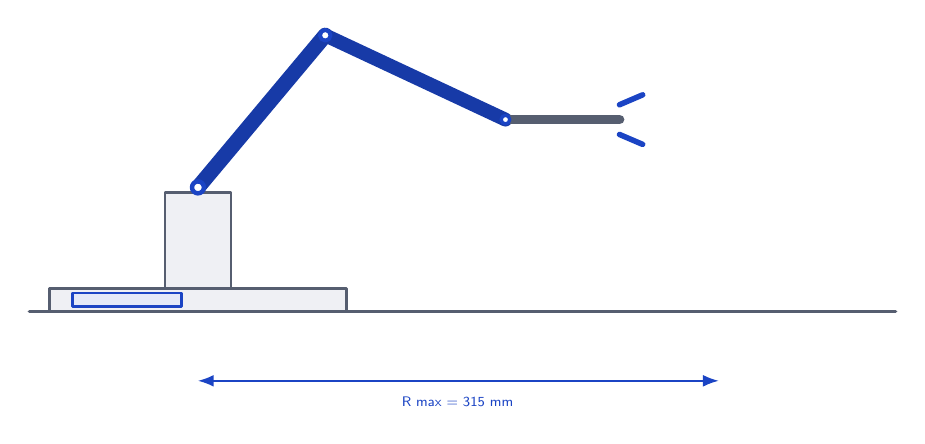
\begin{tikzpicture}[scale=0.021, line cap=round, line join=round]
  % table
  \draw[armgrey, line width=1.2] (8,-330) -- (532,-330);
  % base
  \filldraw[fill=armrule!40, draw=armgrey, line width=1] (20,-330) rectangle (200,-316);
  \filldraw[fill=armblue!12, draw=armblue, line width=0.9] (34,-327) rectangle (100,-319);
  \filldraw[fill=armrule!40, draw=armgrey, line width=1] (90,-316) rectangle (130,-258);
  % links
  \draw[armblue!85!black, line width=5.5] (110,-255) -- (187,-163);
  \draw[armblue!85!black, line width=5.0] (187,-163) -- (296,-214);
  \draw[armgrey, line width=3.5] (296,-214) -- (365,-214);
  \draw[armblue, line width=2] (365,-205) -- (379,-199);
  \draw[armblue, line width=2] (365,-223) -- (379,-229);
  % joints
  \filldraw[fill=white, draw=armblue, line width=1.6] (110,-255) circle (3.6);
  \filldraw[fill=white, draw=armblue, line width=1.4] (187,-163) circle (3.2);
  \filldraw[fill=white, draw=armblue, line width=1.2] (296,-214) circle (2.6);
  % reach dimension
  \draw[armblue, line width=0.6, {Latex}-{Latex}] (110,-372) -- (425,-372);
  \node[below, armblue, font=\tiny\sffamily] at (267,-376) {R max = 315 mm};
\end{tikzpicture}

\vspace{1.6cm}
{\large\bfseries Configuration B --- Recommended} \\[0.2cm]
{\color{armgrey} 315~mm reach \textbullet\ 55~g payload \textbullet\ shoulder safety factor 2.44 \textbullet\ \textasciitilde CAD \$59}

\vfill
{\color{armgrey}\small Prepared as the Phase 1 design review and build reference. \\
Engineering numbers verified against \code{calculations/engineering_calcs.py}. \\
\today}

\end{titlepage}

\tableofcontents
\newpage

% =======================================================================
\section{Executive summary}
% =======================================================================

\textbf{Build Configuration B.} Direct-drive revolute arm, equal 120~mm links, 315~mm reach, 55~g design payload. MG996R at the shoulder and elbow, MG90S at the base and gripper, an SG90 slaved as a wrist leveller, ESP32 over USB serial. Worst-case shoulder safety factor is \textbf{2.44}. Purchase cost \textbf{\textasciitilde CAD~\$59} with typical university-lab sourcing (\$93 worst case, buying everything --- still under the \$100 ceiling).

Two things the arithmetic changes about the design, not just describes:

\begin{itemize}
\item \textbf{The base tips over without ballast.} 224~g of moving arm on a 211~mm lever beats a 269~g base on a 90~mm lever (tipping safety factor 0.89). A 400~g ballast cavity in the base plate fixes it (safety factor 2.22) --- see \S\ref{sec:stability}.
\item \textbf{Do not thicken the printed links.} Tip deflection is 0.075~mm against \textasciitilde6~mm of servo backlash --- the structure is already about 80\texttimes\ stiffer than the servos it is bolted to. Added material there costs shoulder margin for no measurable stiffness benefit --- see \S\ref{sec:mechanical}.
\end{itemize}

Configuration A (ultra-budget, 275~mm reach, \$48--55) is viable but saves only \textasciitilde\$8 over B for a materially smaller robot. Configuration D (stronger actuators, \$85--95) is not justified --- every joint in Configuration B already clears the SF~$\geq 2.0$ floor with margin. Full comparison in \S\ref{sec:configs}.

% =======================================================================
\section{Requirements}
\label{sec:req}
% =======================================================================

\subsection{Scope}
V1 is a mechanically and electronically functional 3-DOF arm, controlled manually or programmatically from a PC over USB. No camera, no vision, no AI agent --- that is V2 (\S\ref{sec:v2}), and V1's software is only required not to block it.

\subsection{Degrees of freedom}
\begin{enumerate}
\item \textbf{Base yaw} --- rotates the whole arm about a vertical axis.
\item \textbf{Shoulder} --- raises/lowers the upper arm in the vertical plane the base currently points at.
\item \textbf{Elbow} --- folds the forearm relative to the upper arm, same plane.
\item \textbf{Gripper} (not a positioning DOF) --- opens/closes a two-finger claw.
\item \textbf{Wrist pitch} --- present in hardware (an SG90) but \emph{not} an independently commanded axis. Firmware slaves it to $-(\theta_1+\theta_2)$ so the gripper stays level in every pose (\S\ref{sec:kinematics}).
\end{enumerate}

This is a positioner with 3 controllable spatial DOF $(x,y,z)$ plus grip --- matching the brief exactly, no more.

\subsection{Target dimensions}
\begin{center}
\begin{tabular}{lcc}
\toprule
\textbf{Parameter} & \textbf{Target (brief)} & \textbf{Chosen} \\
\midrule
Base footprint & 150--200~mm & 180~$\times$~180~mm \\
Reach & 250--350~mm & 315~mm kinematic / 290~mm practical \\
Overall height & 250--400~mm & \textasciitilde340~mm (arm vertical, incl.\ gripper) \\
\bottomrule
\end{tabular}
\end{center}

Link lengths: shoulder height $h_0=75$~mm, upper arm $L_1=120$~mm, forearm $L_2=120$~mm, wrist$\to$TCP $L_3=75$~mm. Equal $L_1=L_2$ is deliberate --- see \S\ref{sec:geometry}.

\subsection{Payload and workspace}
\textbf{Design payload: 55~g} at full 315~mm reach --- pens, small tools, USB sticks, small project boxes, small electronics.

\begin{center}
\begin{tabular}{L{2.6cm}L{2.6cm}L{9.6cm}}
\toprule
\textbf{Bound} & \textbf{Value} & \textbf{Set by} \\
\midrule
Outer radius & 315 / 290~mm & Link length / IK conditioning near full extension \\
Inner radius & 130~mm & Forearm-to-turret collision \\
Floor & $z=10$~mm & Jaw-to-table clearance, enforced in firmware \\
Ceiling & $z=315$~mm & Arm vertical \\
Base sweep & $\pm90\degsym$ & No slip ring in V1 \\
\bottomrule
\end{tabular}
\end{center}

Usable desk area: an annular sector, 130--290~mm radius, 180\degsym\ --- about 0.09~m$^2$ directly in front of the base.

\subsection{Budget}
Target personal spend \textbf{CAD \$50--70}; absolute maximum \textbf{CAD \$100}. Configuration B lands at \textbf{\textasciitilde\$59} with typical lab sourcing, \textbf{\textasciitilde\$93} buying everything. Full breakdown in \S\ref{sec:bom}.

\subsection{Decision gate}
Four questions, answered before any implementation started:
\begin{enumerate}
\item \textbf{Configuration B}, built up from A rather than starting at D.
\item \textbf{SG90 slaved wrist: in.} \$3 and 17~g buys a level gripper in every pose.
\item \textbf{University sourcing:} assume lab-available for controller, bench power supply, fasteners, wire, bearings, filament; budget the MG996R pair and MG90S/SG90 as purchased.
\item \textbf{315~mm / 55~g is the right target} --- no known heavier payload requirement.
\end{enumerate}

% =======================================================================
\section{Architecture}
% =======================================================================

Serial revolute arm --- the classic RRR shoulder--elbow chain on a rotating turret. Base yaw is the only vertical axis; shoulder and elbow work in a single vertical plane the base sweeps around. This is the simplest structure that reaches every point on a desk, and the kinematics collapse to one trig problem.

\begin{center}
\small
\begin{tabular}{@{}L{2.1cm}L{2.3cm}L{2.6cm}L{1.5cm}L{5.4cm}@{}}
\toprule
\textbf{Axis} & \textbf{Type} & \textbf{Range} & \textbf{Actuator} & \textbf{Notes} \\
\midrule
1 --- Base yaw & Revolute, vertical & $-90\degsym\ldots+90\degsym$ & MG90S & Turret on 2$\times$608ZZ bearings \\
2 --- Shoulder & Revolute, horiz.\ & $0\degsym\ldots110\degsym$ & MG996R & Highest-loaded joint \\
3 --- Elbow & Revolute, horiz.\ & $-130\degsym\ldots0\degsym$ & MG996R & Elbow-up solution only \\
Wrist (slaved) & Revolute, horiz.\ & $-120\degsym\ldots+30\degsym$ & SG90 & Firmware-computed, not commanded \\
Gripper & Two-finger, meshed & 0--55~mm & MG90S & Compliant tip \\
\bottomrule
\end{tabular}
\end{center}

\subsection{Why a slaved wrist rather than a parallelogram linkage}
A three-DOF positioner has exactly enough freedom to hit an $(x,y,z)$ target and none left over --- gripper pitch is whatever the IK happens to produce, swinging roughly 30\degsym\ across the workspace. Three ways to fix that:

\begin{description}[leftmargin=1.4em,style=nextline]
\item[Twin parallelogram] Two four-bar linkages hold the jaws level with no extra servo, and move the elbow actuator to the turret. Elegant, but six more printed parts and twelve more pivots with slop at every one. \emph{Deferred.}
\item[SG90 slaved wrist --- chosen] One extra micro servo, driven by firmware as a dependent axis. Costs \textasciitilde\$3 and 17~g at 250~mm, which drops shoulder SF from 2.57 to 2.44 --- cheap for level jaws.
\item[Fixed bracket] Bolt the gripper on at a fixed 45\degsym. Zero cost, zero parts, works if objects are always approached from the side. \emph{Configuration A fallback.}
\end{description}

All three bolt to the same 24$\times$24~mm wrist mounting face on the forearm --- start with the fixed bracket, add the SG90 later, try the linkage after that, without touching another part in the assembly.

% =======================================================================
\section{Geometry}
\label{sec:geometry}
% =======================================================================

Equal-length links, $L_1=L_2=120$~mm --- deliberate, not arbitrary: equal lengths make the printed parts nearly identical (one parametric sketch, two configurations), maximise the folded-to-extended reach ratio, and put the workspace's inner boundary where the turret already is. Every dimension traces back to the torque budget in \S\ref{sec:actuators}.

\begin{figure}[h]
\centering
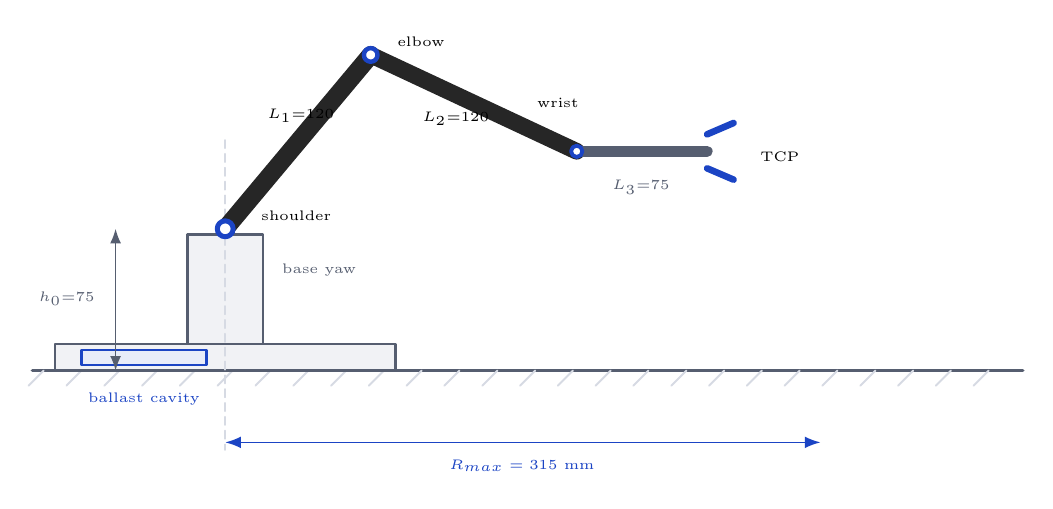
\begin{tikzpicture}[scale=0.024, line cap=round, line join=round, font=\sffamily]
  % table + hatching
  \draw[armgrey, line width=1.3] (8,-330) -- (532,-330);
  \foreach \x in {14,34,...,514} { \draw[armrule, line width=0.7] (\x,-330) -- (\x-8,-338); }
  % base + column
  \filldraw[fill=armrule!35, draw=armgrey, line width=1] (20,-330) rectangle (200,-316);
  \filldraw[fill=armblue!10, draw=armblue, line width=0.9] (34,-327) rectangle (100,-319);
  \node[armblue, font=\tiny] at (67,-345) {ballast cavity};
  \filldraw[fill=armrule!35, draw=armgrey, line width=1] (90,-316) rectangle (130,-258);
  \draw[armrule, line width=0.6, dash pattern=on 3pt off 2pt] (110,-208) -- (110,-372);
  % links
  \draw[black!85, line width=6.5] (110,-255) -- (187,-163);
  \draw[black!85, line width=6.0] (187,-163) -- (296,-214);
  \draw[armgrey, line width=4.0] (296,-214) -- (365,-214);
  \draw[armblue, line width=2.4] (365,-205) -- (379,-199);
  \draw[armblue, line width=2.4] (365,-223) -- (379,-229);
  \filldraw[fill=white, draw=armblue, line width=1.8] (110,-255) circle (4.2);
  \filldraw[fill=white, draw=armblue, line width=1.6] (187,-163) circle (3.6);
  \filldraw[fill=white, draw=armblue, line width=1.4] (296,-214) circle (3.0);
  % labels
  \node[anchor=west, font=\tiny] at (124,-248) {shoulder};
  \node[anchor=west, font=\tiny] at (196,-156) {elbow};
  \node[anchor=south, font=\tiny] at (286,-196) {wrist};
  \node[anchor=west, font=\tiny] at (388,-217) {TCP};
  \node[anchor=west, font=\tiny, armgrey] at (135,-277) {base yaw};
  % dims
  \draw[armgrey, line width=0.5, {Latex}-{Latex}] (52,-255) -- (52,-330);
  \node[anchor=east, font=\tiny, armgrey] at (46,-292) {$h_0{=}75$};
  \node[font=\tiny] at (150,-195) {$L_1{=}120$};
  \node[font=\tiny] at (232,-197) {$L_2{=}120$};
  \node[font=\tiny, armgrey] at (330,-233) {$L_3{=}75$};
  \draw[armblue, line width=0.6, {Latex}-{Latex}] (110,-368) -- (425,-368);
  \node[below, armblue, font=\tiny] at (267,-372) {$R_{max} = 315$~mm};
\end{tikzpicture}
\caption{Side elevation, 1~px~=~1~mm, arm shown mid-stroke. The wrist stays level in every pose, so $L_3$ is a purely horizontal offset in the kinematics.}
\label{fig:elevation}
\end{figure}

\begin{center}
\begin{tabular}{L{3.4cm}L{2.6cm}L{9.0cm}}
\toprule
\textbf{Parameter} & \textbf{Value} & \textbf{Rationale} \\
\midrule
Shoulder height $h_0$ & 75~mm & Elbow folds without hitting the turret \\
Upper arm $L_1$ & 120~mm & Torque-driven --- 140~mm drops shoulder SF below 2.1 \\
Forearm $L_2$ & 120~mm & Equal to $L_1$ --- same printed profile \\
Wrist$\to$TCP $L_3$ & 75~mm & Jaw depth + clearance for a 30~mm object \\
Max TCP reach & 315~mm & Within the 250--350~mm brief \\
Base footprint & 180$\times$180~mm & Drives the tipping calculation, \S\ref{sec:stability} \\
Jaw opening & 0--55~mm & Pen through small project box \\
\bottomrule
\end{tabular}
\end{center}

% =======================================================================
\section{Actuator selection}
\label{sec:actuators}
% =======================================================================

\subsection{Method}
Static gravity-holding torque at the worst-case pose (fully extended, horizontal --- also the normal working pose for a desk arm reaching across the table). Dynamic terms are small at the speeds this arm moves at (under 10\% of the gravity term at the firmware's 60\degsym/s slew limit) and are absorbed by the safety-factor floor rather than modelled explicitly. Target safety factor: \textbf{$\geq 2.0$}, evaluated at 6.0~V rated torque --- roughly the point below which a hobby servo holding a static pose runs hot instead of idling near stall current.

\subsection{Mass budget}
Horizontal distance from the shoulder axis, arm fully extended --- the worst case for every load in the chain. Verified by \code{calculations/engineering_calcs.py}.

\begin{center}
\begin{tabular}{lrrr}
\toprule
\textbf{Item} & \textbf{Mass} & \textbf{Distance} & \textbf{Moment} \\
\midrule
Upper-arm link pair + spacers & 30~g & 60~mm & 1{,}800~g\textperiodcentered mm \\
Elbow servo (MG996R) + bracket & 65~g & 120~mm & 7{,}800~g\textperiodcentered mm \\
Forearm link pair + spacers & 25~g & 180~mm & 4{,}500~g\textperiodcentered mm \\
Wrist servo (SG90) + bracket & 17~g & 250~mm & 4{,}250~g\textperiodcentered mm \\
Gripper assembly (MG90S + jaws) & 32~g & 285~mm & 9{,}120~g\textperiodcentered mm \\
Design payload & 55~g & 320~mm & 17{,}600~g\textperiodcentered mm \\
\midrule
\textbf{Moving assembly total} & \textbf{224~g} & CoM 201~mm & \textbf{45{,}070~g\textperiodcentered mm} \\
\bottomrule
\end{tabular}
\end{center}

Below the shoulder (drives base stability, not shoulder torque): base plate 100~g, column + turret 60~g, base servo 14~g, shoulder servo 55~g, hardware 40~g $\to$ \textbf{269~g}.

The elbow servo alone is 29\% of the moving mass, sitting at the point in the chain where moving it costs the most shoulder torque --- the highest-leverage future change, if shoulder margin ever becomes a problem, is relocating it to the turret behind a linkage (\textasciitilde1.4~kg\textperiodcentered cm), not implemented in V1.

\subsection{Torque calculations}
\begin{align*}
\text{Shoulder: } \tau_1 &= g\sum_i m_i d_i = 9.81 \times 0.04507~\text{kg\,m} = 0.442~\text{N\,m} = 4.51~\text{kg\textperiodcentered cm} \\[4pt]
\text{Elbow: } \tau_2 &= 9.81\times(0.025{\times}0.060 + 0.017{\times}0.130 + 0.032{\times}0.165 + 0.055{\times}0.200) \\
&= 9.81 \times 0.01999 = 0.196~\text{N\,m} = 2.00~\text{kg\textperiodcentered cm} \\[4pt]
\text{Base yaw: } \tau_0 &\approx I\alpha + \text{drag} = 0.0056\times3.5 + \text{drag} \approx 0.30~\text{kg\textperiodcentered cm} \\[4pt]
\text{Wrist: } \tau_3 &= g\left[0.032(0.285{-}0.240) + 0.055(0.320{-}0.240)\right] = 0.057~\text{N\,m} = 0.58~\text{kg\textperiodcentered cm}
\end{align*}

\subsection{Servo table}
\begin{center}
\begin{tabular}{lllrrrl}
\toprule
\textbf{Joint} & \textbf{Servo} & & \textbf{Req.} & \textbf{Target $\times2$} & \textbf{Rated @6V} & \textbf{SF} \\
\midrule
Base & MG90S & & 0.30 & 0.60 & 2.20 & 7.34 \okmark \\
\textbf{Shoulder} & \textbf{MG996R} & \emph{(sizing joint)} & \textbf{4.51} & \textbf{9.02} & \textbf{11.00} & \textbf{2.44} \okmark \\
Elbow & MG996R & & 2.00 & 4.00 & 11.00 & 5.50 \okmark \\
Wrist (slave) & SG90 & & 0.58 & 1.17 & 1.80 & 3.08 \okmark \\
Gripper & MG90S & & 0.82 & 1.64 & 2.20 & 2.70 \okmark \\
\bottomrule
\end{tabular}
\end{center}
\emph{All kg\textperiodcentered cm. On a 5~V supply the MG996R drops to \textasciitilde9.4~kg\textperiodcentered cm and shoulder SF falls to 2.08 --- still acceptable, which is why a 5~V/3~A phone charger is a legitimate power fallback (\S\ref{sec:power}).}

\textbf{Why the elbow is over-specified (SF~5.50), deliberately:} it needs 2.00~kg\textperiodcentered cm, so at SF~2 it needs 4.0. The MG90S tops out at 2.2 and fails. The next rung up, an MG92B at 3.5~kg\textperiodcentered cm (\textasciitilde\$8), still gives only SF~1.75 --- and costs more than an MG996R. The MG996R wins by default and the margin is free.

\subsection{Gripper: SG90 vs MG90S}
Required clamp force for a 55~g object, $\mu=0.5$ (rubber pad, conservative): $mg/2\mu = 0.54$~N. Design target: \textbf{4~N per jaw} --- about 7$\times$ the physics minimum, because real grips are off-centre and objects get bumped.

\begin{align*}
\text{Jaw pivot torque} &= 4.0~\text{N} \times 0.030~\text{m} = 0.12~\text{N\,m} \\
\text{Servo torque (1.5:1 reduction)} &= 0.12 / 1.5 = 0.080~\text{N\,m} = 0.82~\text{kg\textperiodcentered cm}
\end{align*}

\begin{center}
\begin{tabular}{L{2.2cm}L{6.4cm}L{6.4cm}}
\toprule
 & \textbf{SG90} & \textbf{MG90S (chosen)} \\
\midrule
Mass / cost & 9~g / \textasciitilde\$2 & 13.4~g / \textasciitilde\$6 \\
Gears & Nylon --- strips on a hard stall & Metal --- survives stalls/knocks \\
Footprint & 22.8$\times$12.2$\times$22.5~mm, 32~mm span & \textbf{Identical} --- drop-in either way \\
\bottomrule
\end{tabular}
\end{center}

Both pass on torque. The decision is about what happens the twentieth time the gripper closes on something it cannot close on --- metal gears survive it, nylon eventually strips. The identical footprint means the mount is one printed part regardless of which servo goes in it.

\textbf{Mechanism:} two mirror-image printed jaws on M3 pins with meshed gear sectors (module 1.5, \textasciitilde10 teeth engaged) --- one servo drives one jaw, the sectors force the other to mirror it. Self-centring, cannot desync. Jaw faces carry a 90\degsym\ V-groove plus a rubber pad. \textbf{Compliance matters more than gear material:} thin the last 12~mm of each jaw to 1.6~mm so it flexes \textasciitilde1~mm under load --- one commanded ``closed'' angle then grips a range of object sizes without ever driving the servo into a hard stall.

% =======================================================================
\section{Base stability}
\label{sec:stability}
% =======================================================================

Tipping about the front edge of the base plate, arm fully extended, payload at maximum reach. The shoulder axis sits 10~mm forward of the base axis, so the moving CoM is 211~mm out.

\begin{align*}
M_{\text{over}} &= 0.224 \times 9.81 \times (0.211 - 0.090) = 0.266~\text{N\,m} \\[4pt]
M_{\text{rest, no ballast}} &= 0.269 \times 9.81 \times 0.090 = 0.238~\text{N\,m} \quad\Rightarrow\quad \text{SF} = 0.89 \quad \badmark \\[4pt]
M_{\text{rest, +400 g ballast}} &= 0.669 \times 9.81 \times 0.090 = 0.591~\text{N\,m} \quad\Rightarrow\quad \text{SF} = 2.22 \quad \okmark
\end{align*}

\textbf{The arm as drawn tips over.} 224~g on a 211~mm lever beats a 269~g base on a 90~mm lever, and no amount of careful printing fixes that --- it is easy to miss on paper because the whole robot only weighs \textasciitilde500~g.

\subsection{Fixes}
\begin{description}[leftmargin=1.4em,style=nextline]
\item[Ballast the base --- primary] Seal a 66$\times$66$\times$18~mm cavity into the base plate with a snap lid. Fill with washers, sand, or spare screws. \textbf{400~g minimum, 500~g preferred.} Costs nothing and lowers the CoM as well as raising the mass.
\item[Park the supply on the plate] A 6~V~3~A brick weighs 150--250~g. Recessed behind the column, it becomes free ballast plus shorter power leads.
\item[Clamp it down --- optional] Two 8~mm slots at the rear take a small C-clamp. Makes tipping structurally impossible, worth having for fast moves, but should not be the only thing keeping the arm upright.
\end{description}

\textbf{Dynamic loading is worse than this static calculation.} Decelerating the arm at the end of a fast reach adds an inertial term this analysis ignores --- the target is SF~2.2, not 1.2, and firmware slew-limits every joint to 60\degsym/s for exactly this reason.

% =======================================================================
\section{Kinematics}
\label{sec:kinematics}
% =======================================================================

No DH tables, no Jacobians, no numerical solver. Base rotation decouples completely from shoulder/elbow, leaving a two-link planar problem with a closed-form solution --- implemented in \code{software/robot/kinematics.py} (\textasciitilde40 lines including workspace checks, with a self-test that reproduces every number in this section).

\subsection{Forward kinematics}
\begin{align*}
r &= L_1\cos\theta_1 + L_2\cos(\theta_1{+}\theta_2) + L_3 \\
z &= h_0 + L_1\sin\theta_1 + L_2\sin(\theta_1{+}\theta_2) \\
x &= r\cos\theta_0 \qquad y = r\sin\theta_0
\end{align*}
$L_3$ adds directly to $r$ with no trig term --- the payoff of the levelled wrist. Without it, $L_3$ would carry a $\cos(\theta_1{+}\theta_2{+}\theta_3)$ factor and the inverse problem stops being closed-form.

\subsection{Inverse kinematics}
\begin{align*}
\theta_0 &= \operatorname{atan2}(y, x) \\[2pt]
r' &= \sqrt{x^2+y^2} - L_3 \qquad z' = z - h_0 \\[2pt]
D &= \frac{r'^2 + z'^2 - L_1^2 - L_2^2}{2 L_1 L_2} \qquad \text{(unreachable if } |D| > 1\text{, checked before acos)} \\[2pt]
\theta_2 &= -\arccos(D) \qquad \text{(negative root = elbow-up)} \\[2pt]
\theta_1 &= \operatorname{atan2}(z', r') - \operatorname{atan2}\!\big(L_2\sin\theta_2,\ L_1+L_2\cos\theta_2\big) \\[2pt]
\theta_3 &= -(\theta_1+\theta_2) \qquad \text{(slaved wrist, jaws level)}
\end{align*}

The two $\arccos$ roots are elbow-up and elbow-down. Elbow-down puts the elbow below the table on nearly every desk-height target, so the solver takes the negative root unconditionally.

\subsection{Validation order, before anything moves}
\begin{enumerate}
\item \textbf{Reachability} --- $|D|\leq 1$ and $130 \leq \sqrt{x^2+y^2} \leq 290$~mm.
\item \textbf{Joint limits} --- every $\theta$ inside its mechanical range (\S3.2).
\item \textbf{Table clearance} --- $z \geq 10$~mm, and the elbow itself above the table.
\item \textbf{Path check} --- for a Cartesian move, interpolate 20 waypoints and validate each; a straight line between two legal poses can pass through an illegal one.
\end{enumerate}

\textbf{The accuracy limit is backlash, not mathematics.} An MG996R has 1--2\degsym\ of gear lash plus potentiometer deadband. At the 240~mm shoulder+elbow lever, 1.5\degsym\ is \textbf{6~mm at the gripper}. Expect \textbf{$\pm$5--8~mm} repeatability and design around it: approach every target from the same direction, and let the 55~mm jaw opening absorb the rest. No amount of IK precision buys back a millimetre of this.

% =======================================================================
\section{Electronics}
\label{sec:elec}
% =======================================================================

\begin{center}
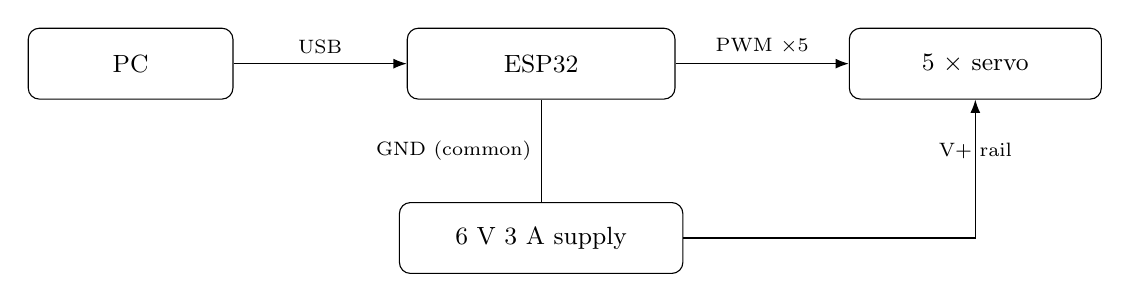
\begin{tikzpicture}[font=\small, node distance=1.4cm, >=Latex]
  \node[draw, rounded corners, minimum width=2.6cm, minimum height=0.9cm] (pc) {PC};
  \node[draw, rounded corners, minimum width=3.4cm, minimum height=0.9cm, right=2.2cm of pc] (nano) {ESP32};
  \node[draw, rounded corners, minimum width=3.2cm, minimum height=0.9cm, right=2.2cm of nano] (servos) {5 $\times$ servo};
  \node[draw, rounded corners, minimum width=3.6cm, minimum height=0.9cm, below=1.3cm of nano] (psu) {6~V 3~A supply};
  \draw[->] (pc) -- node[above,font=\scriptsize]{USB} (nano);
  \draw[->] (nano) -- node[above,font=\scriptsize]{PWM $\times$5} (servos);
  \draw[->] (psu) -| node[above,font=\scriptsize,pos=0.75]{V+ rail} (servos);
  \draw[-] (psu) -- node[left,font=\scriptsize]{GND (common)} (nano);
\end{tikzpicture}
\end{center}

\subsection{Controller: ESP32 (DevKitC or equivalent)}
Full pin-out, colour-coded nets and the grounding/power checklist below are also drawn out as a standalone diagram, \code{wiring_diagram.svg}, alongside this guide. Revised from an original Arduino Nano choice. The Nano's advantage was native \textbf{5~V logic} --- hobby servos want a 5~V pulse, and a 3.3~V board introduces a question with no clean answer on paper: some servos latch reliably on 3.3~V, some jitter, and the difference only shows up after assembly. In practice, the SG90/MG90S/MG996R family used here decodes PWM through an analog RC input stage that a 3.3~V high clears --- a well-worn combination, not a gamble. \textbf{Test each servo before final assembly}; the documented fallback for a unit that jitters is a 74HCT125/74AHCT125 quad buffer (\textasciitilde\$1, covers all five signal lines), not a controller change. In exchange for accepting that one check: a dual-core chip with far more flash/RAM/GPIO than this project needs, a similar street price to the Nano, and Wi-Fi/BT already on board if a future V2 ever wants the arm untethered (unused, not required, by \code{docs/v2_ai_roadmap.md}). Requires the \code{ESP32Servo} library in place of the stock \code{Servo.h} (the ESP32 Arduino core ships neither) --- the \code{attach()}/\code{writeMicroseconds()} API is unchanged, it just rides the chip's LEDC PWM peripheral instead of a hardware timer.

\textbf{Deliberately not included:} a PCA9685 driver board (five servos fit on five ESP32 GPIOs already --- the board solves a problem that starts around twelve servos); encoders or current sensing (hobby servos have no position-feedback path to expose); limit switches (servos are absolute-position devices and already know where they are at power-on).

\textbf{Fallback:} an Arduino Nano/Uno remains a straightforward substitute if an ESP32 isn't available, or a servo won't settle at 3.3~V even behind a level shifter --- same pin roles, same serial protocol, swap \code{ESP32Servo} back for stock \code{Servo.h} and drop the timer-allocation calls in \code{setup()}.

\subsection{Serial protocol}
ASCII, line-oriented, one command per line, every command answered.

\begin{center}
\begin{tabular}{L{4.2cm}L{4.0cm}L{6.8cm}}
\toprule
\textbf{Command} & \textbf{Reply} & \textbf{Purpose} \\
\midrule
\code{PING} & \code{OK ARM v1} & Port identification and liveness \\
\code{J <base> <sh> <el>} & \code{OK} / \code{ERR LIMIT <joint>} & Absolute joint angles, degrees \\
\code{G <0-100>} & \code{OK} & Gripper, 0 closed, 100 open \\
\code{US <ch> <us>} & \code{OK} / \code{ERR RANGE} & Raw pulse, \code{ch}=B/S/E/W/G, calibration only \\
\code{HOME} & \code{OK} & Slew to the safe folded pose \\
\code{STOP} & \code{OK} & Freeze at the current position \\
\code{REL} & \code{OK} & Detach all servos \\
\code{STAT} & angles + \code{us} & Current commanded state \\
\bottomrule
\end{tabular}
\end{center}

The split is deliberate: \textbf{the firmware owns safety, the PC owns intelligence.} Joint limits and slew limiting live on the ESP32 and cannot be bypassed by a buggy Python script --- or, later, a confused AI agent.

% =======================================================================
\section{Power system}
\label{sec:power}
% =======================================================================

\begin{center}
\begin{tabular}{lrrrr}
\toprule
\textbf{Servo} & \textbf{Qty} & \textbf{Idle} & \textbf{Moving} & \textbf{Stall} \\
\midrule
MG996R & 2 & 0.17~A & 0.6--0.9~A & 2.5~A \\
MG90S & 2 & 0.08~A & 0.2--0.4~A & 0.7~A \\
SG90 & 1 & 0.06~A & 0.2~A & 0.65~A \\
\midrule
\textbf{Rail total} & 5 & \textbf{0.56~A} & \textbf{1.2--1.8~A} & \textbf{7.05~A} \\
\bottomrule
\end{tabular}
\end{center}

The 7.05~A all-stall figure is not a design case --- it requires every joint jammed simultaneously. The design case is \textbf{1.8~A continuous, \textasciitilde3.5~A transient} at direction reversals.

\textbf{Specification: 6.0~V, 3~A regulated (18~W), barrel jack, 3~A fuse.} 6.0~V because MG996R torque is quoted at 6~V; at 5~V shoulder SF falls from 2.44 to 2.08. Bulk capacitance: 2$\times$1000~\micro F at the servo headers. $C\Delta V/I = 2000~\micro\text{F}\times0.5\text{V}/2\text{A} = 0.5$~ms --- enough to kill a switching spike, \emph{not} a substitute for a supply that can source the current.

\textbf{Rejected: 4$\times$AA batteries.} Nominal voltage is fine --- 4 fresh alkaline cells land around 6.4~V, inside the 4.8--6.6~V window --- but internal resistance is not: alkaline AAs run \textasciitilde0.15--0.3~$\Omega$ each, so \textasciitilde0.6--1.2~$\Omega$ for the pack. At the 1.8~A design-case draw that is 1.1--2.2~V of sag before the 3.5~A transient case makes it worse --- the same failure mode as the capacitor note above, a source that cannot hold voltage under real load. NiMH cells have lower internal resistance and are the better chemistry if a battery pack is ever used for real, but even then treat it as good for a single-joint bench check, not for running the assembled arm.

\textbf{Three rules, each of which has ended someone's project:} never feed the servo rail from the ESP32's 5V/VIN pin or USB (that pin sits upstream of the board's own 3.3~V logic regulator and reflects whatever the USB port can source, typically \textasciitilde500~mA; five servos will brown it out mid-move); servo ground and ESP32 ground must be joined, or the PWM has no reference and servos twitch randomly; no 7.4~V LiPo direct to the rail --- it will destroy the MG90S and SG90 within minutes.

% =======================================================================
\section{Software architecture}
% =======================================================================

\begin{center}
\begin{tabular}{L{5.6cm}L{9.4cm}}
\toprule
\textbf{Layer} & \textbf{Owns} \\
\midrule
\code{firmware/arm_firmware/} (Arduino C++) & Joint limits, slew rate --- \emph{safety} \\
\code{software/robot/} (Python) & Kinematics, trajectory, transport, the \code{Arm} API \\
\code{software/cli.py}, \code{sequences.py} & Manual control and demo/test routines \\
\emph{V2 (not built)} & \code{software/vision/}, \code{software/agent/} --- add here only \\
\bottomrule
\end{tabular}
\end{center}

The public surface everything else is meant to use --- the CLI, the demo sequences, and eventually the V2 agent --- is \code{robot.arm.Arm}:

\begin{quote}\ttfamily\small
arm.home()\\
arm.move\_joints(base, shoulder, elbow)\\
arm.move\_to(x, y, z)\quad\rmfamily\itshape\small (Cartesian, validated, interpolated)\\
\ttfamily arm.grip(percent)\\
arm.pickup(x, y, z)\\
arm.place(x, y, z)
\end{quote}

This is the V1$\to$V2 contract (\S\ref{sec:v2}): in V2 the agent does not get its own motion code, its own limits, or its own IK --- it calls exactly these six methods. No ROS, no behaviour trees, no message bus --- a 300~mm desk arm with five servos does not have a software problem that a Python class cannot solve.

% =======================================================================
\section{Mechanical design and printing}
\label{sec:mechanical}
% =======================================================================

Links are twin printed side plates on printed spacers --- a box section that is stiff in bending, prints flat with no supports, and puts every bolt in double shear. Roughly 14 unique parts, 20 printed pieces, \textasciitilde300~g of filament, 18--22~h print time.

\subsection{Material assignment}
\begin{center}
\begin{tabular}{L{3.8cm}L{1.6cm}L{9.6cm}}
\toprule
\textbf{Part} & \textbf{Material} & \textbf{Why} \\
\midrule
Base, column, turret & PLA & Stiffness and flatness; not impact-loaded \\
Upper arm, forearm links & PLA & $E\approx3.5$~GPa vs.\ PETG's 2.0 --- deflection matters most \\
Shoulder / elbow brackets & PETG & Highest bending stress; layer adhesion matters most \\
Servo horn adapters & PETG & Small, bolted, loaded to peel layers apart \\
Gripper jaws & PETG & Designed to flex; PLA would snap at the flex section \\
Spacers, clips, tray & PLA & Unloaded \\
Ballast block & Mild steel, milled & Not printed --- see below \\
\bottomrule
\end{tabular}
\end{center}
Print settings: 0.4~mm nozzle, 0.2~mm layers, \textbf{4 perimeters}, 30\% gyroid, 5 top/bottom --- perimeter count dominates strength in a thin printed part.

\subsection{Ballast}
A solid milled block, not loose fill --- a fixed, known mass at a fixed position matches the stability calc's assumption exactly and cannot shift the CoM as the base rotates. \textbf{Mild steel, \textasciitilde50--55~cm\textsuperscript{3} for the 400~g target} ($\rho\approx7.85$~g/cm\textsuperscript{3}): a 60$\times$60$\times$15~mm block is \textasciitilde424~g, clearing the minimum with margin. Steel over aluminium specifically for the footprint --- aluminium ($\rho\approx2.70$) needs \textasciitilde3$\times$ the volume for the same mass, and the ballast cavity already competes for space with the column and base-servo mount inside the 180$\times$180~mm base. Weigh the actual cut block and trim (or size up the blank) to clear 400~g --- mild steel density varies enough between alloys (7.75--7.87~g/cm\textsuperscript{3}) that this is measure-don't-assume, same as everything else safety-factor-adjacent in this guide. Bolt or press-fit it into the cavity; a block free to slide during base rotation turns a designed-in stability margin into an unmeasured one.

\subsection{Layer orientation --- three rules that decide whether this works}
\begin{enumerate}
\item \textbf{Print brackets flat, never standing up.} Loaded perpendicular to the layer planes, a printed part manages only \textasciitilde40--60\% of its in-plane strength.
\item \textbf{Every bolt hole axis is normal to the build plate.} Bolts then clamp \emph{across} layers in compression, not trying to split them apart.
\item \textbf{Never print a servo spline.} A printed 25-tooth spline \emph{will} round off. Bolt the metal horn that shipped with the servo to the printed part with 2--3~M2 screws --- the single most common failure mode in printed arms, designed out from part one.
\end{enumerate}

\subsection{Where FEA earns its time}
\textbf{Worth running (2 studies):} the shoulder bracket (0.44~N\,m through a bolted interface, stress concentration at the servo cutout --- the one part where intuition is unreliable); the upper-arm link's elbow-servo pocket (expect the answer to be ``add a 3~mm fillet''). \textbf{Not worth running:} everything else --- the hand calculation below already answers the question.

\begin{align*}
I &= 2\times\frac{3\times20^3}{12} = 4000~\text{mm}^4 \\
\delta &= \frac{FL^3}{3EI} = \frac{1.3 \times 120^3}{3\times2500\times4000} = 0.075~\text{mm}
\end{align*}

\textbf{Seventy-five microns.} The structure is \textasciitilde80$\times$ stiffer than the servo backlash it is bolted to (\S\ref{sec:kinematics}). \textbf{Do not thicken these links} --- every gram added buys nothing measurable and costs shoulder safety factor directly.

\subsection{Parametric strategy}
One global variables file drives $L_1$, $L_2$, $L_3$, $h_0$, plate thickness and pin diameter across every part. A servo-pocket library feature with a two-row design table (standard: MG996R-class, 40.7$\times$19.7$\times$42.9~mm; micro: MG90S/SG90-class, 22.8$\times$12.2$\times$22.5~mm) means swapping servo sizes is a configuration change, not a redesign --- this is what makes Configurations A--D one robot instead of four. 0.2~mm nominal clearance on every pin and pocket, tuned once via a printed tolerance coupon. Full part list and file layout in \code{cad/README.md}.

% =======================================================================
\section{Bill of materials}
\label{sec:bom}
% =======================================================================

\subsection{BOM A --- purchase}
\begin{center}
\small
\begin{tabular}{L{6.4cm}rrL{4.4cm}}
\toprule
\textbf{Item} & \textbf{Qty} & \textbf{Cost} & \textbf{Likely in a lab?} \\
\midrule
MG996R servo & 2 & \$17 & Unlikely \\
MG90S servo & 2 & \$13 & Maybe \\
SG90 servo & 1 & \$3 & Likely \\
6~V 3~A adapter + barrel jack & 1 & \$14 & Likely (bench PSU substitutes) \\
ESP32 DevKit (CP2102/CH340) & 1 & \$12 & Maybe --- a Nano works as a \$9 fallback \\
1000~\micro F 16~V electrolytic $\times$2 & 1 & \$3 & Very likely \\
608ZZ bearing $\times$2 & 1 & \$4 & Likely \\
M3 screw/nyloc assortment & 1 kit & \$11 & Very likely \\
Dupont wire + perfboard & 1 & \$8 & Very likely \\
PLA + PETG filament (\textasciitilde300~g) & --- & \$8 & Likely \\
\midrule
\textbf{Buy absolutely everything} & & \textbf{\$93} & \emph{under the \$100 ceiling} \\
\bottomrule
\end{tabular}
\end{center}

\emph{Optional, not in the total above:} a 74HCT125/74AHCT125 level shifter (\textasciitilde\$1) if a servo jitters on the ESP32's 3.3~V signal (\S\ref{sec:power}) --- most builds won't need it.

\subsection{BOM B --- university-sourced}
\begin{center}
\small
\begin{tabular}{L{7.2cm}rL{5.4cm}}
\toprule
\textbf{Component} & \textbf{Saves} & \textbf{Substitution risk} \\
\midrule
Microcontroller (ESP32, or Uno/Nano/Mega/Pico fallback) & \$12 & Low --- confirm servo signal quality \\
Power supply (bench PSU) & \$14 & None --- better for testing \\
Fasteners (workshop M3 stock) & \$11 & None \\
Wiring, headers, perfboard & \$8 & None \\
Bearings (mechanism-lab stock) & \$4 & Low \\
Filament (makerspace stock) & \$8 & None \\
Capacitors & \$3 & None \\
Micro servos (teaching kits) & \$16 & Check for stripped gears first \\
\textbf{MG996R $\times$2} & \$17 & \textbf{Plan to buy} --- unlikely on the shelf \\
Ballast stock (mild steel remnant, milled to size, \S\ref{sec:mechanical}) & \$5--8 & Low --- any mild steel blank $\geq$55~cm\textsuperscript{3} works \\
\bottomrule
\end{tabular}
\end{center}

\subsection{Cost summary}
\begin{center}
\begin{tabular}{lr}
\toprule
\textbf{Scenario} & \textbf{Cost} \\
\midrule
Buy everything (worst case) & \$93 \\
\textbf{Typical student (servos + supply + filament, rest sourced)} & \textbf{\$59} \\
Well-stocked lab (MG996R + MG90S only) & \$33 \\
AliExpress route (buy-everything, 3-week wait) & \$42 \\
\bottomrule
\end{tabular}
\end{center}

The \$59 typical-student figure is unaffected by the ESP32 swap --- the controller is lab-sourced in that scenario either way. The AliExpress total moves by only \$1 despite the \$3 Amazon.ca delta, since ESP32 dev boards are inexpensive there too, often \$5--6.

% =======================================================================
\section{Configuration comparison}
\label{sec:configs}
% =======================================================================

\begin{center}
\small
\setlength{\tabcolsep}{3.5pt}
\begin{tabular}{L{2.2cm}L{2.9cm}L{2.9cm}L{2.9cm}L{2.9cm}}
\toprule
 & \textbf{A --- Ultra-budget} & \textbf{B --- Recommended} & \textbf{C --- University} & \textbf{D --- Stronger} \\
\midrule
Purchase cost & \$48--55 & \$55--65 & \$17--35 & \$85--95 \\
Reach & 275~mm & 315~mm & 315~mm & 315~mm \\
Payload & 30~g & 55~g & 55~g & 80~g \\
Base & SG90 & MG90S & lab micro servo & MG90S \\
Shoulder & MG996R & MG996R & MG996R & DS3218 (20~kg\textperiodcentered cm) \\
Elbow & MG90S & MG996R & MG996R & MG996R \\
Gripper & SG90 & MG90S & MG90S & MG90S \\
Wrist & fixed bracket & SG90 slaved & SG90 slaved & MG90S slaved \\
Shoulder SF & 4.1 & 2.44 & 2.44 & 4.0 \\
University components & minimal & minimal & \textbf{high} & optional \\
\bottomrule
\end{tabular}
\end{center}

Every column is the \emph{same robot}: same CAD files, same assembly, same firmware, same Python. A$\to$B is a 40~mm forearm configuration change and two servo swaps. B$\to$D is one servo and a different mounting plate.

\subsection{Decision trail}
\begin{description}[leftmargin=1.4em,style=nextline]
\item[G1 --- Can the cheapest configuration meet torque requirements?] Yes, but only at 275~mm reach and 30~g payload --- satisfies torque by shrinking the robot to the low end of the brief's range. \emph{Conditional pass.}
\item[G2 --- Can university components close the gap at zero cost?] Partly --- \textasciitilde\$45 of the BOM is plausible lab stock, but MG996R-class servos usually are not. \emph{Partial.}
\item[G3 --- Is the step from A to B worth its cost?] Yes, decisively: \$8 buys +40~mm reach, +25~g payload, and a levelled wrist. \textbf{Configuration B selected.}
\item[G4 --- Does B leave enough margin, or is D required?] Every joint clears SF~2.0. A DS3218 would add \$18 to fix a problem that does not exist. \textbf{Configuration D not required.}
\end{description}

% =======================================================================
\section{Component fallbacks}
% =======================================================================

\begin{center}
\small
\begin{tabular}{L{2.1cm}L{2.6cm}L{3.5cm}L{2.6cm}L{3.5cm}}
\toprule
\textbf{Component} & \textbf{Primary} & \textbf{If unavailable} & \textbf{If too weak} & \textbf{University} \\
\midrule
Shoulder & MG996R & MG995 & DS3218 & Any 9--20~kg\textperiodcentered cm servo \\
Elbow & MG996R & MG90S + $L_2{=}80$mm & 2nd MG996R & Standard-frame servo \\
Base & MG90S & SG90 & MG996R & Any micro servo \\
Gripper & MG90S & SG90 + lighter jaws & MG92B & Check for stripped gears \\
Wrist & SG90 & fixed 45\degsym\ bracket & MG90S & Any micro servo \\
Controller & ESP32 & Nano/Uno (5V) & --- & ESP32/Uno/Nano/Pico \\
Power & 6V 3A adapter & 5V 3A charger ($-$15\%) & 6V 5A adapter & Bench supply \\
\bottomrule
\end{tabular}
\end{center}

\subsection{Geometry fallback --- apply strictly in this order}
\begin{enumerate}
\item \textbf{Cut the payload} --- 55~g$\to$30~g removes 39\% of the shoulder moment for free.
\item \textbf{Shorten the forearm} --- $L_2$ 120$\to$80~mm, reach falls to 275~mm.
\item \textbf{Lighten the prints} --- 3~mm$\to$2.5~mm plates, 30\%$\to$20\% infill; \textasciitilde12~g saved, deflection stays under 0.15~mm.
\item \textbf{Only then, a bigger servo} --- and re-check steps 1--3 first.
\end{enumerate}

A 350~mm arm at 55~g needs \textasciitilde5.4~kg\textperiodcentered cm at the shoulder --- an MG996R right at the edge, or \$18 more for a DS3218. The 315~mm arm clears 4.51 comfortably on the \$8 servo. 35~mm of reach is not worth doubling the actuator budget.

% =======================================================================
\section{Design risks}
% =======================================================================

\begin{center}
\small
\begin{tabular}{@{}p{4.6cm}lp{7.6cm}@{}}
\toprule
\textbf{Risk} & \textbf{Severity} & \textbf{Mitigation} \\
\midrule
Printed servo-horn interface strips & \badmark & Never print splines --- bolt the metal horn on. Designed in from part one. \\
Base tips forward & \badmark & 400~g ballast cavity + supply on the plate (\S\ref{sec:stability}). Verify by hand before power-on. \\
Brownout resets mid-move & \badmark & Separate 3~A servo rail, common ground, 2$\times$1000~\micro F, never the ESP32's 5V/VIN pin. \\
Servo jitters on ESP32's 3.3~V signal & \warnmark & Test each servo before final assembly; add a 74HCT125 level shifter (\textasciitilde\$1) on that signal line, or fall back to a Nano (\S\ref{sec:bom}) --- see \S Controller in Electronics. \\
Backlash limits accuracy to \(\pm\)6~mm & \warnmark & Unfixable in software --- approach from one direction, rely on jaw opening. \\
Gripper servo cooks while holding & \warnmark & Compliant jaw tips + \code{REL} to detach after a grip is established. \\
Arm driven into the table & \warnmark & Firmware clamps independently of the PC; software validates every waypoint. \\
Print tolerances bind the joints & \warnmark & 0.2~mm nominal clearance; print a tolerance coupon first. \\
Servo buzz at rest & \okmark & Detach on idle via \code{REL} --- cosmetic. \\
PLA creep under sustained load & \okmark & Deflection is 0.075~mm at 5\% of yield --- don't park extended for days. \\
\bottomrule
\end{tabular}
\end{center}

% =======================================================================
\section{Build timeline}
% =======================================================================

Assumes 6--10~h/week alongside coursework.

\begin{center}
\small
\begin{tabular}{@{}cp{2.6cm}p{3.6cm}p{6.4cm}@{}}
\toprule
\textbf{Week} & \textbf{Phase} & \textbf{Output} & \textbf{Done when} \\
\midrule
0 & Requirements & This guide, signed off & Configuration chosen, order placed \\
1--2 & Mechanical design & SolidWorks parts + assembly & Assembly rebuilds cleanly when $L_1$ changes \\
2--3 & Print & \textasciitilde20 parts, 300~g & Everything fits without a file; budget 2 revisions \\
3 & Assembly + wiring & Arm on the desk & Every joint moves freely by hand \\
4 & Firmware & Serial protocol, limits, slew & Each joint sweeps its range without binding \\
5 & Kinematics + calibration & Python layer, \code{arm.py} & \code{move\_to()} lands within $\pm$8~mm \\
6 & Testing & Payload, repeatability, thermal & Picks and places a pen 10 times running \\
7 & Documentation & README, docs/, CAD exported & Someone else could rebuild it from the repo \\
\bottomrule
\end{tabular}
\end{center}

\textbf{6--8 weeks part-time.} Phase 5 calibration is where schedules slip --- per-servo microsecond offsets take a patient evening.

% =======================================================================
\section{V1 $\to$ V2 roadmap}
\label{sec:v2}
% =======================================================================

Nothing here gets built now --- it is recorded so V1's decisions do not close a door V2 needs open.

\begin{center}
\small
\begin{tabular}{L{2.3cm}L{5.0cm}L{1.1cm}L{5.6cm}}
\toprule
\textbf{Stage} & \textbf{Adds} & \textbf{Cost} & \textbf{Touches V1?} \\
\midrule
2.1 Eyes & USB webcam on a printed overhead mast & \$0--15 & One new printed part \\
2.2 Desk-plane calibration & Four-point homography: pixels $\to$ desk coords & \$0 & New module --- the whole coordinate problem, since the desk is flat \\
2.3 Detection & YOLO / colour-contour detector $\to$ centroids & \$0 & New module \\
2.4 Agent & LLM with \code{arm.pickup()}/\code{arm.place()} as tools & \$0 & \textbf{Nothing} --- same six calls the CLI uses \\
\bottomrule
\end{tabular}
\end{center}

\textbf{Three decisions V1 makes on V2's behalf}, each free now and expensive to retrofit: the PC holds intelligence and the MCU holds safety, so an agent physically cannot exceed a joint limit; the arm's public API is Cartesian, so vision output plugs straight in; the base plate has camera-mast mounting provision, so the camera-to-robot transform calibrates once and stays valid.

``Pick up my screwdriver and put it beside my laptop'' resolves to: detect $\to$ centroid $\to$ homography $\to$ \code{arm.pickup(x,y,z)} $\to$ agent picks a target $\to$ \code{arm.place(x',y',z')}. Every step after the homography is V1 code that already works.

\subsection{Payload upgrade path --- gearmotors + encoders (a separate track)}
A different axis from the AI stages above: actuation/payload, not perception. Not part of ``V2'' as the brief scoped it (vision/AI on an \emph{unchanged} chassis) --- recorded separately so it is not implied by, or confused with, the AI stages. Hobby servos are closed-loop internally and absolute-position at power-on; DC gearmotors are not, so this swap needs an encoder + PID position loop per joint in firmware (new work, not a config change), a homing routine (reversing the ``servos are absolute-position, no limit switches needed'' decision in \S\ref{sec:elec}), a motor driver per joint in place of direct PWM-to-servo wiring, a power budget redone from scratch (\S\ref{sec:power}), and a new mechanical design sized for gearmotor+gearbox envelopes rather than micro servos. What does \emph{not} change: \code{robot.arm.Arm}'s six public calls and the Cartesian API contract, since that boundary was already drawn actuator-agnostic. Not scoped or budgeted yet --- needs its own design review (motor/gear/encoder/driver selection) before it is a real plan, the same gate V1 went through in \S\ref{sec:req}.

% =======================================================================
\section{Decision gate}
% =======================================================================

Four answers, recorded, that unlock implementation:

\begin{enumerate}
\item \textbf{Configuration B} --- built up from A rather than starting at D.
\item \textbf{SG90 slaved wrist: in} --- \$3 and 17~g for level jaws in every pose.
\item \textbf{University sourcing assumed} for controller, bench supply, fasteners, wire, bearings, filament; MG996R pair and MG90S/SG90 budgeted as purchases.
\item \textbf{315~mm / 55~g} is the design target --- no known heavier payload requirement.
\end{enumerate}

\vspace{0.4cm}
\noindent\textcolor{armgrey}{\small Every figure in this guide is reproduced by \code{calculations/engineering_calcs.py} (self-checking against the values above) and \code{software/robot/kinematics.py} (FK/IK round-trip self-test). Servo ratings are published manufacturer specs for generic parts --- verify against what you actually receive, since MG996R quality varies between sellers.}

\end{document}
